\section{Durchführung}
\label{sec:Durchführung}

Zur Durchführung des Versuchs wird ein Aufbau wie in Abbildung \ref{fig:Aufbau} dargestellt verwendet. Dabei findet der eigentliche Effekt in der Photozelle statt (Abbildung \ref{fig:Photo}). Diese ist ein evakuierter Glaskolben, in dessen Innern sich zwei Elektroden befinden. Eine Elektrode ist dabei eine auf die Innenwand gedampfte Metallschicht. Dazu parallel und mit wenig Abstand ist ein kreisförmiger Drahtring platziert. In diesem Aufbau dient die Metallschicht als Photokathode, auf welche das Licht fällt, und der Drahtring als entprechende Anode. 

\begin{figure}
\centering
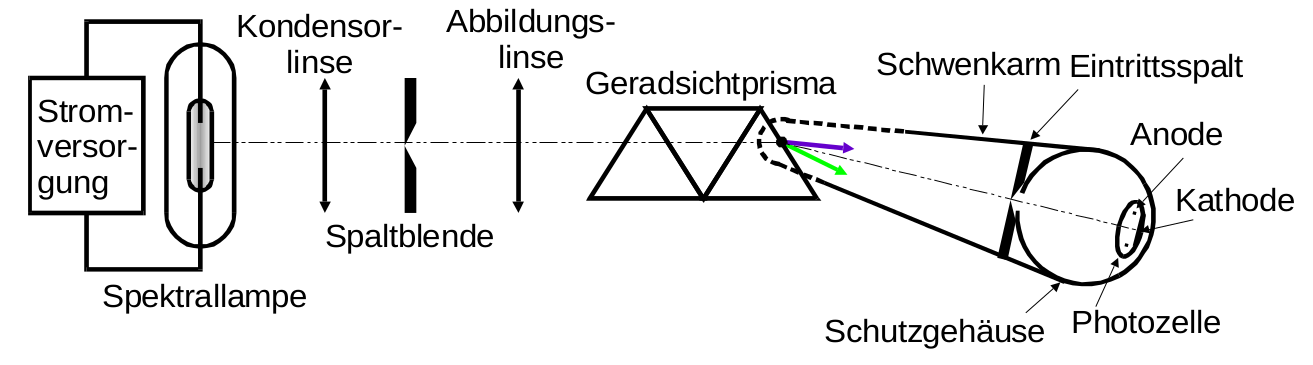
\includegraphics[width=\textwidth]{data/Aufbau.png}
\caption{Aufbau des Versuchs.}
\label{fig:Aufbau}
\end{figure}

\begin{figure}
\centering
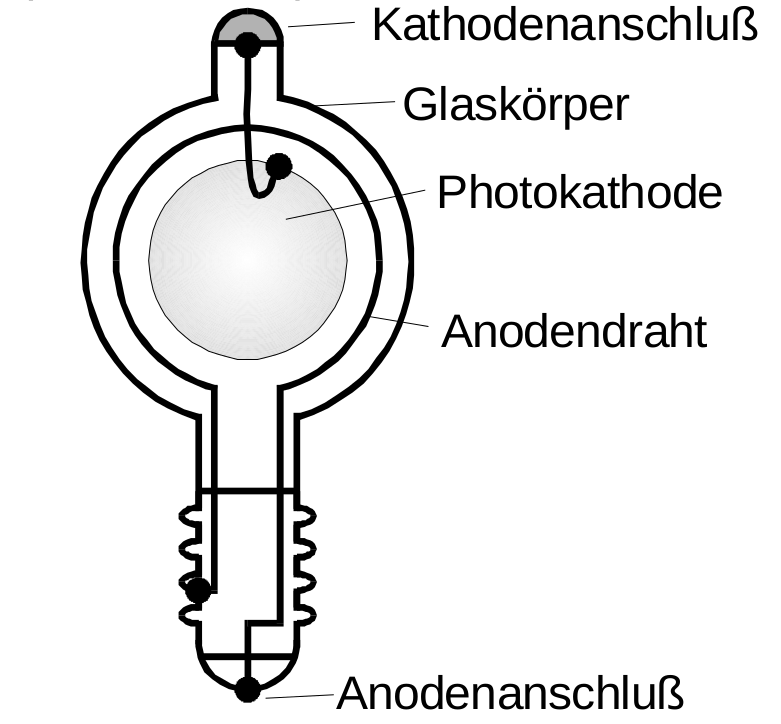
\includegraphics[height=7cm]{data/Photozelle.png}
\caption{Aufbau der Photozelle.}
\label{fig:Photo}
\end{figure}

Das Licht wird von der Hg-Lampe emittiert, von der Kondensatorlinse auf die Spaltblende gebündelt und fällt durch das Geradsichtprisma. Dort wird das Licht räumlich in seine Spektrallinien getrennt. Die Photozelle kann jeweils passend verschoben werden, sodass nur das Licht einer Spektrallinie einfällt. So lässt sich sicherstellen, dass jeweils monochromatisches Licht auf die Photokathode trifft.



Um die Energie der ausgelösten Elektronen zu bestimmen, wird die Gegenfeldmethode verwendet. Dazu wird eine Schaltung gemäß Abbildung \ref{fig:Schaltung} verwendet. Es wird also ein Gegenfeld zwischen Anode und Kathode erzeugt, welches dafür sorgt, dass nicht mehr alle Elektronen die Anode erreichen. Ab einer bestimmten Gegenspannung erreichen keine Elektronen mehr die Anode. Kurz bevor dies geschieht, schaffen es nur noch die schnellsten Elektronen auf die Anode. Desshalb lässt sich für diese Elektronen die Gleichung
\begin{equation}
    e_0 U_g=\frac{1}{2}m_0v_{\text{max}}^2
\end{equation}
aufstellen.

\begin{figure}
\centering
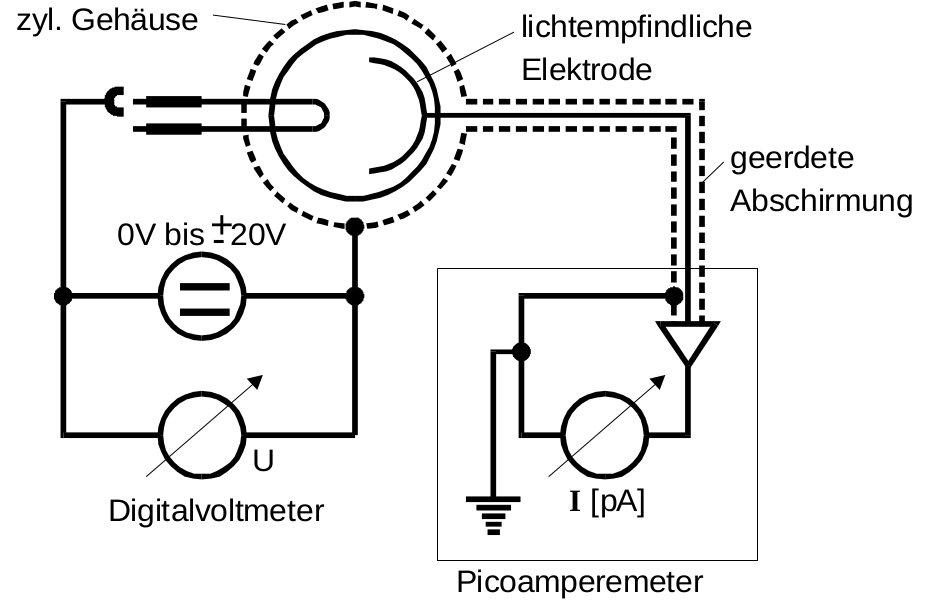
\includegraphics[height=6cm]{data/Schaltung.png}
\caption{Für den Versuch verwendete Schaltung zum Variieren der Gegenspannung.}
\label{fig:Schaltung}
\end{figure}

Daraus ergibt sich für das Photon, welches eines dieser schnellen Elektronen auslösen kann, eine Energie, welche über 
\begin{equation}
    h\nu=e_0 U_G + A_k
\end{equation}
bestimmt werden kann. 

Da jedoch die Elektronen im Festkörper ein breites Spektrum unterschiedelicher Energien besitzen, ist das Verschwinden des Photostroms nicht schlagartig, sondern nähert sich kontinuierlich der Null an. Der ungefähre Kurvenverlauf des Photostroms in Abhängigkeit der Bremsspannung ist in Abbildung \ref{fig:Kurve} dargestellt.

\begin{figure}
\centering
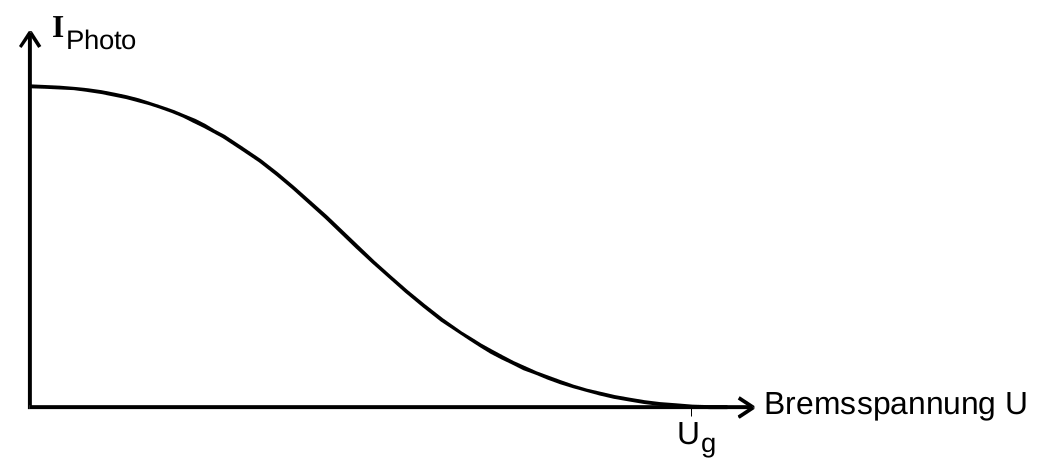
\includegraphics[height=7cm]{data/Kurve.png}
\caption{Prinzipieller Kurvenverlauf des Photostroms in Abhängigkeit der Bremsspannung.}
\label{fig:Kurve}
\end{figure}

Es lässt sich zeigen, dass unter bestimmten Voraussetzungen ein Zusammenhang zwischen Photostrom und Bremsspannung gemäß
\begin{equation}
    I_{\text{Ph}}\sim U^2
\end{equation}
existiert.
Darüber lässt sich $U_g$ bestimmen, in dem $\sqrt{I}$ gegen $U$ aufgetragen wird. Der Schnittpunkt der Gerade mit der $U$-Achse enstpricht $U_g$.

Darüber hinaus kann es unter bestimmen Vorraussetzungen dazu kommen, dass gelöste Elektronen die Anode nicht erreichen, da das Anodenmaterial eine hohe Austrittsarbeit besitz. Die Energieverteilung zwischen Anode und Kathode kann dann so aussehen, wie in Abbildung \ref{fig:Energie} dargestellt ist.
Dadurch kann es dazu kommen, dass bei der verwendeten Photozelle und niedriger Bremsspannung negative Ströme zu beobachten sind. Damit erschwert sich abermals die Bestimmung von $U_g$, da sich dieser Strom mit dem der Kathode überlagert.

\begin{figure}
\centering
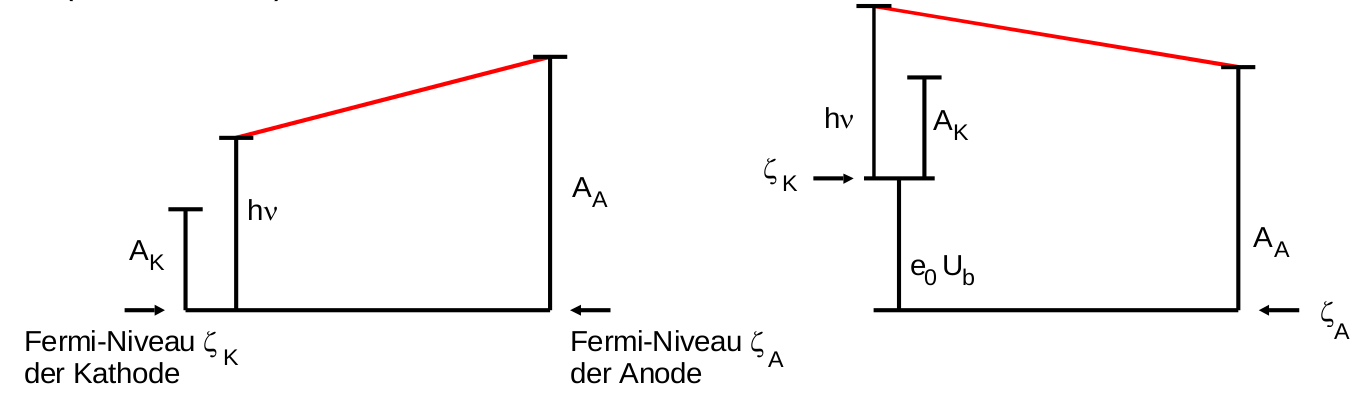
\includegraphics[width=\textwidth]{data/Energie.png}
\caption{Energieniveaus ohne und mit beschleunigendem Potenzial.}
\label{fig:Energie}
\end{figure}


Bei der Versuchsdurchführung wird darüber hinaus auf eine möglichst störfreie Umgebung geachtet. Da es sich bei den vorliegenden Strömen um sehr geringe Ströma handelt, werden Koaxialkabel verwendet. Außerdem wird der Versuch in möglichst absoluter Dunkelheit durchgeführt.














%Was wurde gemessen bzw. welche Größen wurden variiert?